\section{Структура базы данных}

\indent В разрабатываемой базе данных необходимо хранить:

\begin{itemize}
	\item данные о заказах;
	\item данные о типах продукции;
	\item данные о продукции, которая относится к каждому заказу;
	\item данные о самой последовательности операций и самих операциях для каждого типа продукции;
	\item данные о каждой модели ресурсов;
	\item данные о связях между моделью ресурса и операциями.
\end{itemize}

\begin{figure}[ht]
	\centering
	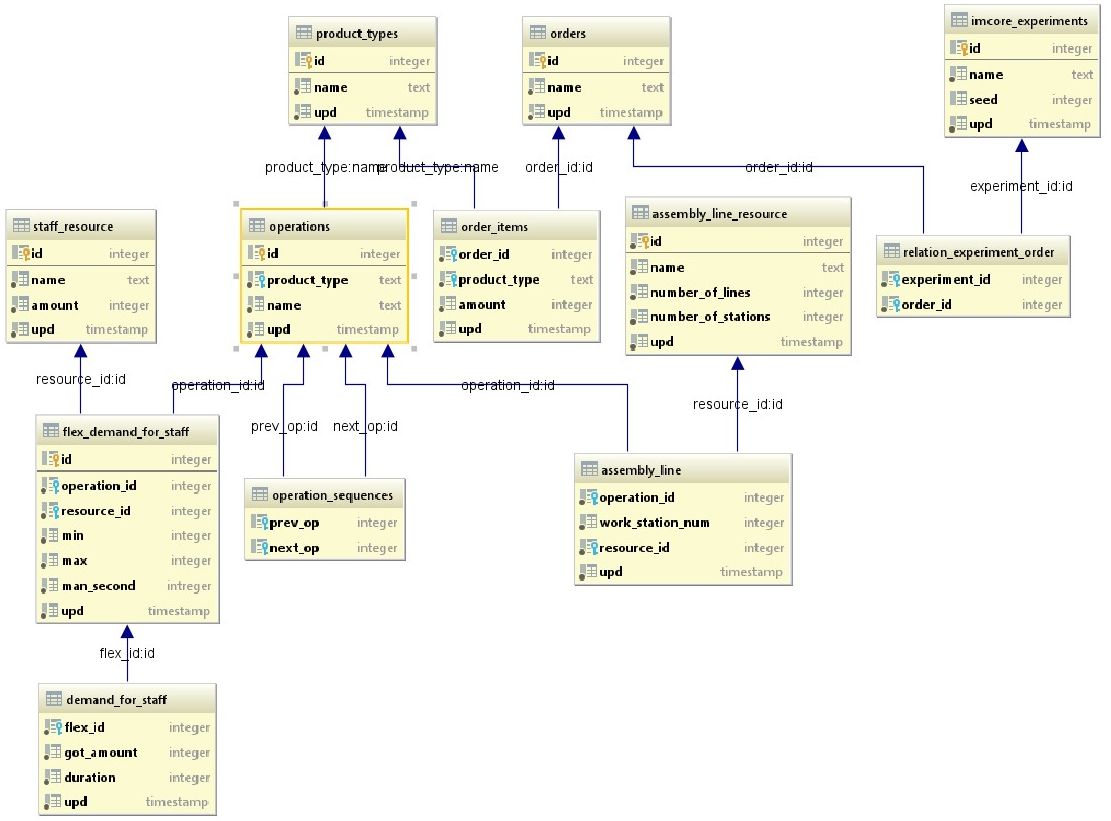
\includegraphics[width=\linewidth]{pics/databaseSchema.png}
	\caption{Схема базы данных}
	\label{fig:dbSchema}
\end{figure}


\indent Помимо этого, нужно учитывать, что кроме простого хранения данных, необходимо соблюдать ``версионность'', ввиду того, что карта технологического процесса может меняться во времени.
Значит и в базе данных требуется следить за тем, чтобы в любой момент времени было возможно использовать любую из версий данной карты, иначе новый расчет оперативного плана (при условии, что другие данные остались неизменными) приведет к созданию новой версии плана, а, следовательно, предыдущую версию восстановить будет либо очень сложно, либо, в худшем случае, невозможно.\\
\indent Для этого, учитывая определенные в разделе \ref{sec:theorem} теоремы и операции, все отношения были разделены две категории: 
\begin{itemize}
	\item внешний ключ является ссылкой на поле уникального идентификатора (id);
	\item внешний ключ является ссылкой на текстовое поле имени (name), а также имеет поле ``version''.
\end{itemize}

\indent Эти типы впоследствии были связаны между собой и позволили создать более гибкую структуру базы данных
С помощью этой метки можно получить как последние данные из базы, просто максимизируя метку ``version'', так и данные на определенный момент времени ограничивая эту метку необходимым временем.